\documentclass[a4paper,12pt]{report}
\usepackage[showexo=true,showcorr=false]{../packages/coursclasse}
%Commenter ou enlever le commentaire sur la ligne suivante pour montrer le niveau
\toggletrue{montrerNiveaux}

%\usepackage{cmbright}
\usepackage{arev}
\usepackage{enumitem}
\setlist[enumerate]{align=left,leftmargin=1cm,itemsep=10pt,parsep=0pt,topsep=0pt,rightmargin=0.5cm}
\setlist[itemize]{align=left,labelsep=1em,leftmargin=*,itemsep=0pt,parsep=0pt,topsep=0pt,rightmargin=0cm}

\setlength\columnsep{35pt}

\begin{document}
%%%%%%%%%%%%%%%%% À MODIFIER POUR CHAQUE SERIE %%%%%%%%%%%%%%%%%%%%%%%%%%%%%
\newcommand{\chapterName}{Nombres et opérations}
\newcommand{\serieName}{Estimer, encadrer \\et placer sur une droite}


%%%%%%%%%%%%%%%%%% PREMIERE PAGE NE PAS MODIFER %%%%%%%%%%%%%%%%%%%%%%%%
% le chapitre en cours, ne pas changer au cours d'une série
\chapter*{\chapterName}
\thispagestyle{empty}

%%%%% LISTE AIDE MEMOIRE %%%%%%
\begin{amL}{\serieName}{
	\item Représentation de nombres décimaux sur une droite graduée (page 21)
\item Définition d'une fraction (page 27)
\item Passage d'une écriture fractionnaire à une écriture décimale (page 28)
\item Passer d'une écriture décimale à une écriture fractionnaire (page 28)
\item Amplification et simplification d'une fraction (page 29)
}
\end{amL}
%%%%%%%%%%%%%%% DEBUT DE LA SERIE NE PAS MODIFIER %%%%%%%%%%%%%%%%%%%%%%%%%%%%%
\section*{\serieName}
\setcounter{page}{1}
\thispagestyle{firstPage}



%%%%%%%%%%% LES EXERCICES %%%%%%%%%%%%%%%%%%%%%%%%%%%%%%%%%%%
\begin{resolu}{Extraire des entiers et reste}{
Combien d'entiers peut-on extraire de chacune des fractions suivantes ?
Quelle fraction reste-t-il ?

 Afin de déterminer combien d'entiers on peut extraire d'une fraction, il faut répondre à la question suivante: \emph{Combien de fois peut-on mettre le dénominateur dans le numérateur?} C'est-à-dire effectuer la division entière du dénominateur par le numérateur. 

\begin{tasks}(1)
	\task $\dfrac{47}{8}:$ On peut mettre cinq fois $8$ dans $47$ et il reste alors $\dfrac{7}{8}$, car $47\div 8=5$ reste $7$. On peut donc extraire $5$ entiers et il reste $\dfrac{7}{8}$.  
	\task $\dfrac{3}{5}:$ On peut mettre zéro fois $3$ dans $5$ et il reste $\dfrac{3}{5}$, car $3\div 5=0$ reste $3$. On peut donc extraire $0$ entier et il reste $\dfrac{3}{5}$. 
	\task $\dfrac{59}{11}:$ On peut extraire $5$ entiers et il reste $\dfrac{4}{11}$. 
\end{tasks}
}{1}
\end{resolu}

\begin{exof}{NO199}{70}{1}
\end{exof}
\begin{exof}{NO200}{70}{2}
\end{exof}

\begin{exo}{
Combien d'entiers peut-on extraire de chacune des fractions suivantes ?
Quelle fraction reste-t-il ?
	\begin{tasks}(3)
\task $\dfrac{4}{3}$
\task $\dfrac{7}{2}$
\task $\dfrac{23}{3}$
\task $\dfrac{18}{5}$
\task $\dfrac{100}{19}$
\task $\dfrac{50}{12}$
\end{tasks}
\vspace{1pt}}
{1}\end{exo}

\begin{exo}{
Combien d'entiers peut-on extraire de chacune des fractions suivantes ?
Quelle fraction reste-t-il ?
	\begin{tasks}(3)
\task $\dfrac{150}{45}$
\task $\dfrac{240}{18}$
\task $\dfrac{99}{6}$
\task $\dfrac{190}{21}$
\task $\dfrac{300}{18}$
\task $\dfrac{900}{22}$
\end{tasks}
\vspace{1pt}}
{1}\end{exo}

\begin{exo}{
De quel nombre naturel ces fractions sont-elles le plus proche?
	\begin{tasks}(3)
\task $\dfrac{13}{3}$
\task $\dfrac{54}{6}$
\task $\dfrac{78}{11}$
\task $\dfrac{21}{2}$
\task $\dfrac{51}{4}$
\task $\dfrac{60}{9}$
\end{tasks}
 \vspace{1pt}
}{2}\end{exo}


\begin{exo}{
De quel nombre naturel ces fractions sont-elles le plus proche?
	\begin{tasks}(3)
\task $\dfrac{80}{11}$
\task $\dfrac{100}{15}$
\task $\dfrac{31}{2}$
\task $\dfrac{476}{9}$
\task $\dfrac{123}{5}$
\task $\dfrac{231}{17}$
\end{tasks}
 \vspace{1pt}
}{2}\end{exo}


\begin{exof}{NO198}{69}{2}
\end{exof}

\begin{qmoodle}{Extraire et encadrer}{2}{
	\begin{center}	
		Q-Extraire le plus grand entier


\includegraphics[scale=1]{media/qr/eepdq1}

\tiny{{https://edu.ge.ch/qr/eepdq1}}
\end{center}
	\begin{center}	
		Q-Encadrer une fraction


\includegraphics[scale=1]{media/qr/eepdq2}

\tiny{{https://edu.ge.ch/qr/eepdq2}}
\end{center}
}
\end{qmoodle}

\begin{exo}{
Encadre les fractions suivantes entre deux nombres consécutifs.
	\begin{tasks}(3)
\task $\dfrac{22}{7}$
\task $\dfrac{12}{17}$
\task $\dfrac{73}{20}$
\task $\dfrac{15}{2}$
\task $\dfrac{30}{4}$
\task $\dfrac{5}{2}$
\end{tasks}
 \vspace{1pt}
}{1}\end{exo}


\begin{exo}{
Encadre les fractions suivantes entre deux nombres consécutifs.
	\begin{tasks}(3)
\task $\dfrac{43}{7}$
\task $\dfrac{29}{3}$
\task $\dfrac{7}{3}$
\task $\dfrac{14}{9}$
\task $\dfrac{58}{9}$
\task $\dfrac{153}{10}$
\end{tasks}
 \vspace{1pt}
}{1}\end{exo}


\begin{exo}{
Encadre les fractions suivantes entre deux dizaines consécutives.
	\begin{tasks}(3)
\task $\dfrac{200}{5}$
\task $\dfrac{120}{9}$
\task $\dfrac{300}{8}$
\task $\dfrac{140}{4}$
\task $\dfrac{210}{3}$
\task $\dfrac{560}{6}$
\end{tasks}
 \vspace{1pt}
}{2}\end{exo}

\begin{exo}{
Encadre les fractions suivantes entre deux dizaines consécutives.
	\begin{tasks}(3)
\task $\dfrac{570}{13}$
\task $\dfrac{4400}{11}$
\task $\dfrac{8480}{5}$
\task $\dfrac{7740}{23}$
\task $\dfrac{1230}{9}$
\task $\dfrac{153}{2}$
\end{tasks}
 \vspace{1pt}
}{2}\end{exo}

\begin{exof}{NO186}{68}{1}
\end{exof}
\begin{exof}{NO187}{68}{3}
\end{exof}
\begin{exof}{NO188}{69}{1}
\end{exof}



\begin{resolu}{Placer des fractions sur une droite}{
Dessine une droite numérique (entre 0 et 10) et places-y le plus précisément possible les nombres suivants.

{\color{blue} On écrit la fraction sous forme décimale avec une précision avec une précision qui dépend de la graduation, puis on place le nombre sur la droite. 
}

\begin{tasks}(1)
	\task $\dfrac{24}{5}=24\div 5=4,8$
	\task $\dfrac{31}{4}=31\div 4=7,75\simeq 7,8$
	\task $\dfrac{-1}{6}=-1\div 6\simeq -0,1\overline{6}$
\end{tasks}
\centering
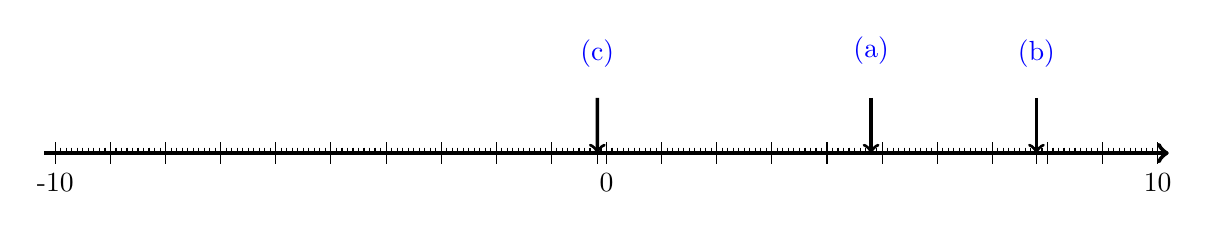
\begin{tikzpicture}[scale=0.7]
  \draw[->,ultra thick] (-10.2,0) -- (10.2,0);
  \foreach \i in {-10,-9,...,10} % numbers on line
    \draw ({10*\i/10},0.2) -- + (0,-0.4) node[below] {}; % tick and their labels
  \draw ({10*(-10)/10},0.2) -- + (0,-0.4) node[below] {-10};
  \draw (0,0.2) -- + (0,-0.4) node[below] {0};
  \draw ({10*(10)/10},0.2) -- + (0,-0.4) node[below] {10};
  \foreach \i in {-100,-99,...,100} % numbers on line
    \draw ({10*\i/100},0.1) -- + (0,-0.1) node[below] {}; % tick and their labels

  % réponses
\draw[very thick][->] (4.8,1) -- (4.8,0);
\draw[very thick][->] (7.8,1) -- (7.8,0);
\draw[very thick][->] (-0.1666,1) -- (-0.16666,0);
  \draw (4.8,0.1) -- + (0,-0.1) node[above=1cm] {\color{blue}(a)};
 \draw (7.8,0.1) -- + (0,-0.3) node[above=1.1cm] {\color{blue}(b)};
 \draw (-0.1666,0.1) -- + (0,-0.3) node[above=1.1cm] {\color{blue}(c)};
\end{tikzpicture}}{1}
\end{resolu}


\begin{exo}{
Dessine une droite numérique (entre 0 et 10) et places-y le plus précisément possible les nombres suivants.
\[
a=6,25 \quad b=\dfrac{7}{2} \quad c=\dfrac{3}{4} \quad d=\dfrac{15}{4} \quad e=2,3 \quad f=\dfrac{23}{10} \quad g=\dfrac{8}{1} \quad h=\dfrac{16}{5}
\]}
{1}\end{exo}

\begin{exo}{
Dessine une droite numérique (entre 0 et 1) et places-y le plus précisément possible les nombres suivants.
\[
a=\dfrac{1}{1} \quad b=\dfrac{1}{2} \quad c=\dfrac{1}{3} \quad d=\dfrac{1}{4} \quad e=\dfrac{1}{5} \quad f=\dfrac{1}{6} \quad g=\dfrac{1}{7}
\]}
{2}\end{exo}

\begin{exo}{
Dessine une droite numérique (entre 0 et 2) et places-y le plus précisément possible les fractions suivantes.
\[
a=\dfrac{2}{3} \quad b=\dfrac{7}{10} \quad c=\dfrac{4}{9} \quad d=\dfrac{7}{5} \quad e=\dfrac{5}{4} \quad f=\dfrac{6}{8}
\]}
{2}\end{exo}




\begin{exol}{NO189}{52}{2}
\end{exol}
\begin{exol}{NO191}{52}{1}
\end{exol}
\begin{exof}{NO204}{71}{1}
\end{exof}
%\exol{NO203}{54}{2}
%\begin{exopn}
%Une consigne {\cursive{{\color{blue}un texte}}}
%\begin{enumerate}
%\medskip\item Le $\;$\hrulefill$\;$ 432 est composé des $\;$\hrulefill$\;$ 2, 3 et 4.
%\end{enumerate}
%\end{exopn}

%\begin{exop}
%Consigne
%\end{exop}


\end{document}
